\section{Benchmarks}\label{sec:benchmarks}
\subsection{Parameters and security estimations}
The constraints to derive the parameters are summarized in Table \ref{tab:constraints}.
We ran a script \footnote{\label{fn:github}\url{https://anonymous.4open.science/r/chipmunk-code-56E6}}
that enumerates all possible 
parameters, in terms of the modulus of the rings, the arity of decomposition, etc., and finds the parameter sets that
allow for smallest signature size. Table \ref{tab:param} summarizes the results from the script. 
\begin{table}
  \centering
  \begin{tabular}{@{\makebox[3em][r]{\rownumber\space}} l@{\hspace{3em}}rl}
  \toprule
   \multicolumn{1}{@{\makebox[3em][r]{\#\space}} c}{Source}&\multicolumn{2}{c}{Constraint}\\
  \midrule
   \autoref{lem:hvcprobhom}&$\bagg \geq$&$ \eta\sqrt{2\alpha_w\rho(\epsilon + 1 + \log_2 n + \log_2(2\tau \lceil\log_{2\eta+1}q\rceil + \xi\lceil\log_{2\eta+1}q'\rceil))\cdot\ln2}$\\
   \autoref{lem:kots_correct}& $\beta_\sigma \geq$&$ 4\varphi\alpha_H\sqrt{\tfrac{1}{2}\alpha_w\rho(\varepsilon+1+\log_2n\gamma)\cdot\ln2}$\\
   \autoref{lem:kots_sis}&$\abs{\tern_{\alpha_H}} \geq$&$ 2^{2\secpar}$\\
   \autoref{lem:keyhidden}& $\gamma\geq$&$((3\secpar+\delta)/n+\log_2q)\log^{-1}_2(\varphi+\tfrac{1}{2})$\\
   \autoref{lem:keyhidden}& $\abs{\tern_{\alpha_H}} \leq$&$ 2^{2\secpar + \delta}$\\
   \autoref{lem:nilssupportivechildsupport}&$q'>$&$ 16 \alpha_w \alpha_H\varphi$\\
   \autoref{lem:msigaggcorrect}&$\chi \geq$ &$\secpar/(\varepsilon-1)$\\
   \autoref{lem:msigunf}&$\abs{\tern_{\alpha_w}} \geq$&$2^\secpar$
  %\bottomrule
  \end{tabular}
  \caption{The constraints a set of Chipmunk parameters needs to satisfy to ensure that the proofs are applicable. The parameters additionally need to be chose such that the associated Ring-SIS problems are hard.}\label{tab:constraints}
  \end{table}
  

We require the ring-SIS problem in Lemma \ref{lem:hvcprobhom} and \ref{lem:kots_correct} to be hard. 
We also require that the hamming weights of the message hashes and the randomizers are sufficient for combinatorial security.
In terms of the lattice security, we use a same approach to derive the security of the parameters as in Squirrel \cite{CCS:FleSimZha22}.
We adopted the so-called ``realistic model'' in \cite{DBLP:conf/uss/AlkimDPS16}.
For a BKZ of block size $\beta$, the cost in this model is estimated by
$2^{0.292\beta+16.4+\log(\#\texttt{SVP calls})}$. 
In the meantime, the LWE-estimator \cite{DBLP:journals/jmc/AlbrechtPS15}
shows that for a root Hermite factor of $1.005$ we expect a block size of 286, which yields 112 bits security under the above model. 

\subsection{Implementations}
We implemented Chipmunk in Rust. We release our source code, as well as the scripts for parameter derivation to the open domain\footnoteref{fn:github}.

\subsubsection{Comparisons}\label{ss:comparison}

We compare the performance of Chipmunk against both the trivial solution, i.e., repeating Falcon signature for $\rho$ times, and
Squirrel \cite{CCS:FleSimZha22}, the previous state-of-the-art. The data for Chipmunk and Squirrel are collected over a same benchmark platform: an AMD 5900x with 24 threads
and 32 Gigabytes of memory. The data for Falcon-512 is collected from their official website\footnote{\url{https://falcon-sign.info/}}.
All three candidates yield 112 bits security.

The comparison with the trivial solution is quite straightforward. Since its signature size grows linearly with the number of signers,
Chipmunk can easily improve by a couple of order of magnitudes when the number of signers increases.
Also note that the signing speed of Chipmunk is of the same order of magnitude as Falcon-512.

In terms of Squirrel, we see that for both $\rho = 1024$ and $\rho = 8192$, our scheme is always better. 
In particular, there were two main obstacles that prevent Squirrel from being widely deployed, namely, the key generation time
and the signature size. We show that the key generation time is improved by a factor of 9 over a same platform; and the 
aggregated signature size is reduced by 5 times. 

\begin{table}\centering
  \begin{tabular}{|c||l|c|c|c||c|c|c|c||c|c|c|}\hline
    \# signers      &                 & Falcon      & Squirrel  & Chipmunk  & Imp. Falcon & Imp. Squirrel \\\hline\hline
    \multirow{2}{*}{} 
                    & Key Generation  & 8.6 ms      & 4 min     & 26.5 sec  &     -       & 9.0$\times$ \\\cline{2-7}
                    & Signing         & 0.17 ms     & 2.1 ms    & 0.4 ms    &     -       & 5.2$\times$ \\\cline{2-7}
                    &Fresh Sig. Size  & 666 Bytes   & 45 KB     & 32 KB     &     -       & 1.4$\times$ \\\hline\hline
    \multirow{3}{*}{1024}                
                    &Aggregation      & -           & 1.2 sec   & 0.55 sec  &     -       & 2.2$\times$ \\\cline{2-7}
                    &Batch Verification    
                                      & 36.7 ms     & 19.5 ms   & 7.2 ms    & 5.1$\times$ & 2.7$\times$ \\\cline{2-7}
                    
                    &Agg. Sig. size   & 682 KB      & 572 KB    & 142 KB    & 4.8$\times$ & 4.0$\times$ \\\hline\hline
    \multirow{3}{*}{8192}                
                    &Aggregation      & -           & 9.6 sec   & 4.3 sec   &     -       & 2.2$\times$ \\\cline{2-7}
                    &Batch Verification    
                                      & 294 ms      & 53  ms    &  47 ms    & 6.2$\times$ & 1.1$\times$ \\\cline{2-7}
                    &Agg. Sig. size   & 5.5 MB      & 762 KB    & 160 KB    & 340$\times$ & 4.8$\times$ \\\hline
  \end{tabular}\\
  Falcon: trivial solution via concatenating ``\# signers''  signatures.\\
  Squirrel and Chipmunk: uses parameters $\lambda = 112$ and $\tau=21$. \\
  \caption{Comparisons among different solutions.}

\end{table}

\subsubsection{Practical performance}
To show that Chipmunk is practical, 
we take a deep dive into the two major obstacles, namely, the key generation time and the aggregated signature size.

We conduct a benchmark over a typical server that is equipped with an AMD 7773x with
64 cores and 1 Terabytes of memory.
The results are summarized in Table \ref{tab:bench_results}.
Notice that this platform is different from that of Section \ref{ss:comparison},
and more accurately simulates the real world node runners for blockchains.

\begin{table}[t]\centering
  \begin{tabular}{|c|c|c|c|c|c|c|c|c||c|c|c|}\hline
      Tree Height         & Key Generation            & Online Signing\footnotemark        
      & $\#$ Signers  
                                                                                            &  Aggregation & Verification  & Agg. Sig. Size  \\ \hline\hline
      \multirow{2}{*}{21} & \multirow{2}{*}{7.4 sec}  & \multirow{2}{*}{0.40 ms}  & 1024    &   491 ms     &  7.3 ms       & 142 KB     \\\cline{4-7}
                          &                           &                           & 8192    &   3.5 sec    &  42.3 ms      & 160 KB     \\\hline\hline

      \multirow{2}{*}{24} & \multirow{2}{*}{1 min}    & \multirow{2}{*}{0.44 ms}  & 1024    &   492 ms     &  7.5 ms       & 160 KB     \\\cline{4-7}
                          &                           &                           & 8192    &   3.8 sec    &  42.1 ms      & 180 KB     \\\hline\hline

      \multirow{2}{*}{26} & \multirow{2}{*}{  4 min}  & \multirow{2}{*}{0.44 ms}  & 1024    &   518 ms     &  7.1 ms       & 172 KB     \\\cline{4-7}
                          &                           &                           & 8192    &   4.0 sec    &  42.9 ms      & 194 KB     \\\hline

  \end{tabular}\\
  \caption{Benchmark results}
  \label{tab:bench_results}
\end{table}
\footnotetext{Similar to \cite{CCS:FleSimZha22}, Chipmunk is also an online-offline signature scheme.
The secret key contains of a merkle tree.
Via caching the top layers of the tree, the signer trades the storage with signing speed.  
Here we report the online signing cost assuming the signer stores the full tree.
} 
% \end{table}
% \subsection{Micro Benchmarks}
We measure the time to generate the keys. As we shall see in Figure \ref{fig:keygen}, the key generation time scales linearly in the 
height of the tree. For the largest parameter set with $\tau = 26$, we can generate a keypair within 4 minutes, improving from 2 hours in Squirrel.
This is sufficient for 21 years of usage, assuming each block takes 10 seconds to finalize as in the case of Ethereum. 
We conclude that the key generation time is no longer a bottleneck for practical deployment.
\begin{figure}[H] 
  \centering
  \begin{subfigure}[b]
  {0.45\textwidth}    \centering
  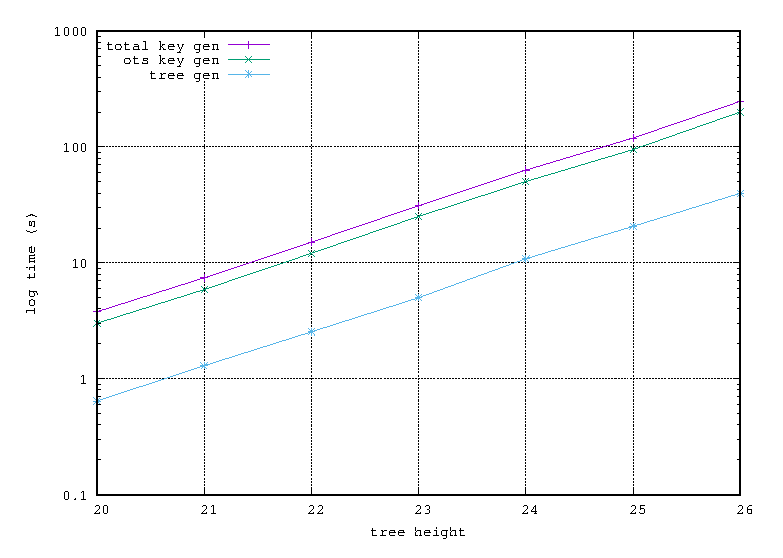
\includegraphics[width=\textwidth]{figures/key_gen.eps}\\
  \caption{Chipmunk key generations.}
  \label{fig:keygen}
  \end{subfigure}
~
\begin{subfigure}[b]{0.45\textwidth}    \centering
  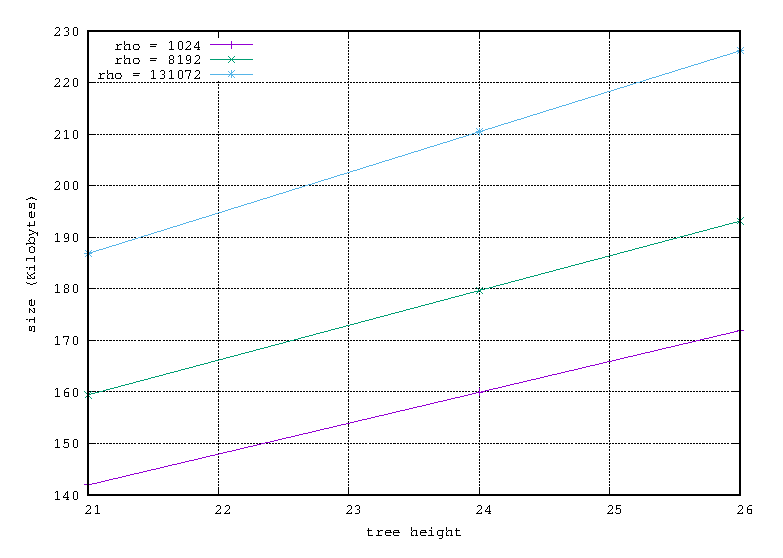
\includegraphics[width=\textwidth]{figures/sig_size.eps}\\
  \caption{Chipmunk aggregated signature size}
  \label{fig:sigize}
  \end{subfigure}

\end{figure}


% \subsection{Sizes}
In terms of the signature size, for the parameter set with $\tau=21$ and $\rho=1024$,
an aggregated signature is of size 142 Kilobytes, consists of 
\begin{itemize}
  \item the aggregated path to the root and its adjacent nodes, i.e., $2\tau\lceil\log(q, \eta)\rceil$ polynomials in $\mathcal{R}_q$ with an infinity norm bound $\beta <2^{15}$. This adds up to $126$ Kilobytes.
  \item the aggregation of decomposed public keys for the one time signature scheme, i.e., $2\lceil\log(q', \eta)\rceil$ polynomials in $\mathcal{R}_{q}$ with norm bound $\beta < 2^{15}$, or $8$ Kilobytes 
  \item the aggregated one time signature, i.e., $\gamma$ polynomials in $\mathcal{R}_{q'}$ with norm bound $\beta_\sigma < 2^{20}$, or $8$ Kilobytes.
\end{itemize}
This almost fits inside a single ethereum block whose peak size is around 130 Kilobytes to date\footnote{\url{https://etherscan.io/chart/blocksize}}.


